
\subsubsection{Explicación}
En este caso escogeremos una técnica greedy diferente.
Para intentar mejorar las estrategias del vecino más cercano y la inserción de vértices nos centraremos en una estrategia que consiste en ir seleccionando las aristas de menor longitud.

Primero crearemos una clase Arista donde guardaremos los índices de los puntos dentro del grafo (índices de ambos vértices de la arista) y la distancia entre ellos, sacada de la matriz de adyacencia del grafo.

Definimos una relación de orden entre aristas de la siguiente forma:
Una arista es \textit{menor que} otra si la distancia entre sus puntos es menor que la distancia entre los puntos de la segunda arista.

Posteriormente ordenaremos todas las aristas en un vector, e iremos seleccionando hasta 
pasar por todos los vértices una única vez, comprobando en cada paso que no forme nuevos ciclos.

\subsubsection{Comprobación de ciclo constante}

Para desarrollar una forma constante para comprobar si una arista forma ciclos o no hemos usado un vector de listas de aristas $vector < list <Edges> >$ .

Cada lista definirá un camino inconexo con el resto de listas del vector, de forma que su primer elemento y último sean los extremos del camino, pasando por los puntos intermedios.
Al final del algoritmo nos quedará una única lista ordenada con la solución.

Para saber si una arista forma ciclo o no asignaremos un estado a cada vértice.
Inicialmente los vértices tienen estado -1, significa que no han sido usados aún por el algoritmo (no están en ninguna lista).

Si se inserta una nueva arista, su primer vértice (inicio del camino) pasará al estado
[1+10*posicion], siendo \textit{posicion} el lugar que ocupa dentro del vector de listas (es una forma de diferenciar los diferentes caminos, necesaria).
De esta forma si (estado1/10 == estado2/10) sabemos que los vértices están en el mismo camino.

El segundo vértice (último elemento) tendrá el estado [2+10*posicion]
            
Si hubiese vértices entre el principio y el final (cuando tenemos más de una arista) los vértices intermedios tendrían estado [3+10*posicion]

Estos casos nos permiten saber directamente al insertar una arista si forma ciclo.




\subsubsection{Casos posibles}
Denotando como \textit{one} y \textit{two} los códigos de los vértices de la arista que queremos insertar.


\textbf{Caso 1(bien)}: Ninguno está. En este caso se añadiría una nueva lista con una sola arista que nos indicaría que se ha creado un nuevo camino,                 en lugar de extender uno anterior.

%#-----------#  *--*

\textbf{Código}: 

\hspace{1cm}((one == -1) \& \& (two == -1))

\textbf{Caso 2(bien)}: Está uno y el otro está libre.
      
%#-----------*--*

\textbf{Código}: 

\hspace{1cm}((one\%10 == 1) \& \& (two == -1) || (one\%10 == 2) \& \& (two == -1)
                 
\hspace{1cm}(two\%10 == 1) \& \& (one == -1) || (two\%10 == 2) \& \& (one == -1) )

 
\textbf{Caso 3(bien)}: La arista une caminos, están los dos vértices, pero en caminos diferentes.

%#-----------*--*----------------------#

Meteremos los elementos de la segunda lista de aristas en la primera
            
\textbf{Código}:

\hspace{1cm}( ((one\%10 == 1) \& \& (two\%10 == 1) \& \& (one/10 != two/10)) ||
                     
\hspace{1cm}((one\%10 == 2) \&\& (two\%10 == 2) \& \& (one/10 != two/10)) ||

\hspace{1cm}((one\%10 == 1) \&\& (two\%10 == 2) \&\& (one/10 != two/10)) ||

\hspace{1cm}((one\%10 == 2) \&\& (two\%10 == 1) \&\& (one/10 != two/10)) )


\textbf{Caso 4(mal)}: Está uno en mitad y otro libre

\textbf{Código}: 

\hspace{1cm}((one == -1 \& \& two\%10 == 3) || (two == -1 \& \& one\%10 == 3))

\textbf{Caso 5(mal)}: Están los dos y forman ciclo

\textbf{Código}: 

\hspace{1cm}( ((one\%10 == 1) || (one\%10 == 2)) \& \& 
\hspace{1cm}((two\%10 == 1) || (two\%10 == 2)) \& \& (one/10 == two/10) )
            
           
\subsubsection{Eficiencia}
Siendo $n$ el número de puntos del grafo, para ordenar las $n^2$ aristas usaremos el Heapsort, por tanto obtenemos una eficiencia de $n^2log(n^2) \implies n^2log(n)$.

En el peor caso recorreremos las $n^2$ aristas hasta encontrar las $n$ aristas deseadas.
Como el algoritmo para ver si una arista forma ciclo es constante, si forma ciclo pasará a la siguiente iteración, si no forma añadirá dicha arista.


\subsubsection{Explicación gráfica}

\begin{figure}[htbH] 
	\centering
	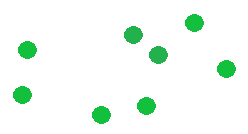
\includegraphics[width=0.5\textwidth]{./Imagenes/arista1.png}
	\caption{Eligiendo punto de inicio en azul} 
\end{figure}

\vspace{0.5cm}
\begin{figure}[htbH] 
	\centering
	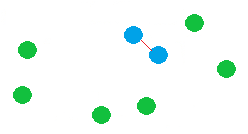
\includegraphics[width=0.5\textwidth]{./Imagenes/arista2.png}
	\caption{Tercer vértice} 
\end{figure}

\vspace{0.5cm}
\begin{figure}[htbH] 
	\centering
	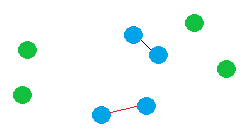
\includegraphics[width=0.5\textwidth]{./Imagenes/arista3.png}
	\caption{Cuarto vértice} 
\end{figure}

\vspace{0.5cm}
\begin{figure}[htbH] 
	\centering
	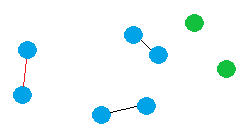
\includegraphics[width=0.5\textwidth]{./Imagenes/arista4.png}
	\caption{Quinto vértice} 
\end{figure}

\vspace{0.5cm}
\begin{figure}[htbH] 
	\centering
	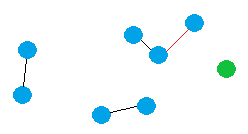
\includegraphics[width=0.5\textwidth]{./Imagenes/arista5.png}
	\caption{Sexto vértice} 
\end{figure}

\vspace{0.5cm}
\begin{figure}[htbH] 
	\centering
	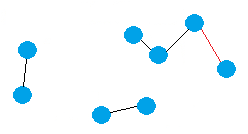
\includegraphics[width=0.5\textwidth]{./Imagenes/arista6.png}
	\caption{Séptimo vértice} 
\end{figure}


\vspace{0.5cm}

Debemos tener en cuenta que solamente podemos unir aristas que estén en dos caminos diferentes si sus puntos son extremos de caminos ya existentes. De esta forma aunque un vértice sea un extremo de un camino, si su otro extremo está en mitad de otro camino no nos vale, ya que llegaría un punto en el que pasaríamos dos veces por el mismo punto.

\begin{figure}[htbH] 
	\centering
	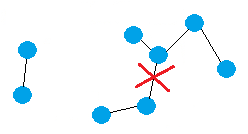
\includegraphics[width=0.5\textwidth]{./Imagenes/arista6fail.png}
	\caption{Octavo y último vértice} 
\end{figure}

\vspace{0.5cm}
\begin{figure}[htbH] 
	\centering
	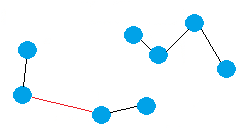
\includegraphics[width=0.5\textwidth]{./Imagenes/arista7.png}
	\caption{Octavo y último vértice} 
\end{figure}

\vspace{0.5cm}
\begin{figure}[htbH] 
	\centering
	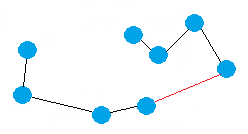
\includegraphics[width=0.5\textwidth]{./Imagenes/arista8.png}
	\caption{Octavo y último vértice} 
\end{figure}

No debemos olvidar terminar el camino.

\begin{figure}[htbH] 
	\centering
	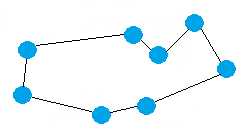
\includegraphics[width=0.5\textwidth]{./Imagenes/arista9.png}
	\caption{Recorrido vecino más cercano} 
\end{figure}

\newpage
\subsubsection{Ejemplos}
Puntos:

	\begin{figure}[htbH]
		\centering
		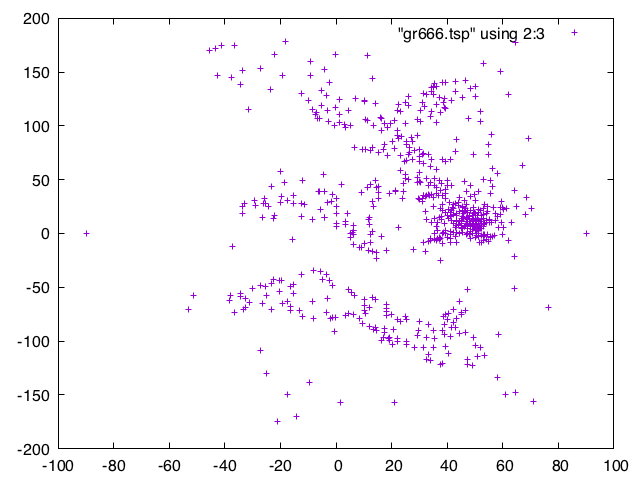
\includegraphics[width=0.65\textwidth]{../Viajante/Imagenes/gr666.png}
		\caption{Quinto vértice}
	\end{figure}
	
Recorrido óptimo:

	\begin{figure}[htbH]
		\centering
		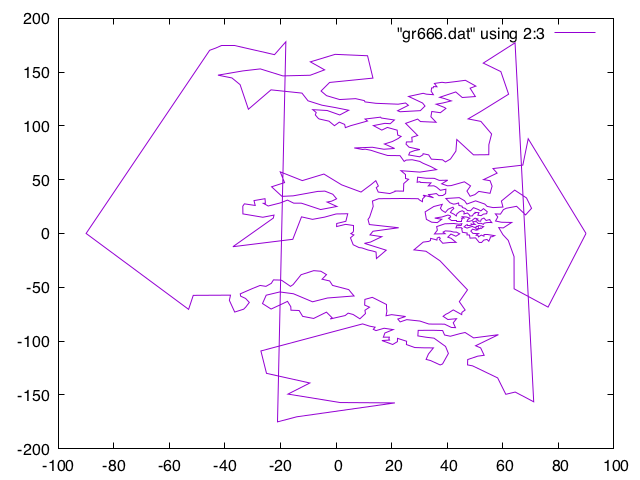
\includegraphics[width=0.65\textwidth]{../Viajante/Imagenes/gr666_opt.png}
		\caption{Quinto vértice}
	\end{figure}
\newpage